%!TEX root = project.tex

\chapter*{About this project}
\paragraph{Abstract}
People often buy items that they only intend to use once, and just throw it in the corner for eternity. Even aside from the one-off purchases, many of people's belongings are barely used by them and are left idle for most of the time. BarterNearMe is a website which offers a solution to this problem in the form of a 21st century barter system. This website provides users with the ability to login, register and browse or add available items and wanted items. The user may also save an available item for later viewing. 

\paragraph{Authors}
Explain here who the authors are. Nathan Garrihy and Cathal Donohoe.

\chapter{Introduction}

The introduction should be about three to five pages long. (5 recommended)
Provide a clear context for your project.
– What is it about? Is it at the right level (8)?
– Is the scope correct?
– Do not assume that the reader knows anything about the domain.
– Why should a reader care or be interested?
q Set out the objectives of the project clearly.
– You will have to address each of these in the evaluation /
conclusion.
– The metrics by which success or failure is measured.
q Briefly list each chapter / section and provide a brief description
of what each section contains.
– List the resource URL (GitHub address) for the project and provide
a brief list and description of the main elements at the URL.
q After reading the introduction, a reader should be 100% certain
of what the project is all about and why it is relevant.
Make sure you use references~\cite{einstein}

\chapter{Context}
(3-5 pages)
Describe the way you went about your project. Was your
approach to the problem valid?
– Software development v/s Research methodology.
q Agile / incremental and iterative approach to development.
– Planning. Did you storyboard? How did you determine the
requirements for the project?
– Meetings. Frequency, structure, checks & balances, feedback.
q What about validation and testing?
– Junit or some other framework.
q If team based, did you use GitHub during the development
process? What about other development tools?
– Selection criteria for algorithms, languages, platforms and
technologies.
q Was an empirical approach used? How were problems solved?
– Was any research undertaken first?
\begin{itemize}
\item Provide a context for your project.
\item Set out the objectives of the project
\item Briefly list each chapter / section and provide a 1-2 line description of what each section contains.
\item List the resource URL (GitHub address) for the project and provide a brief list of the main elements at the URL.
\end{itemize}

\section{Filler}


\subsection{More filler}


\section{Filler}



\chapter{Methodology}
About one to two pages.
Describe the way you went about your project:
\begin{itemize}
\item Agile / incremental and iterative approach to development. Planning, meetings.
\item What about validation and testing? Junit or some other framework.
\item If team based, did you use GitHub during the development process.
\item Selection criteria for algorithms, languages, platforms and technolo-gies.
\end{itemize}
Check out the nice graphs in Figure \ref{tikz:graphs}, and the nice diagram in Figure \ref{tikz:mydiagram}.

\begin{figure}
  \centering
  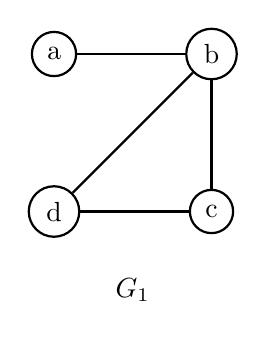
\begin{tikzpicture}
  \begin{scope}[every node/.style={circle,thick,draw}]
  \node (a) at (0,2) {a};
  \node (b) at (2,2) {b};
  \node (c) at (2,0) {c};
  \node (d) at (0,0) {d};
  \end{scope}
  \begin{scope}[every edge/.style={draw=black,thick}]
  \path (a) edge (b);
  \path (b) edge (c);
  \path (b) edge (d);
  \path (c) edge (d);
  \end{scope}
  \node () at (1,-1) {$G_1$};
  \end{tikzpicture}
  \hspace{1.5cm}
  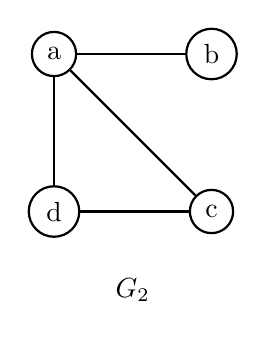
\begin{tikzpicture}
  \begin{scope}[every node/.style={circle,thick,draw}]
  \node (1) at (0,2) {a};
  \node (2) at (2,2) {b};
  \node (3) at (2,0) {c};
  \node (4) at (0,0) {d};
  \end{scope}
  \begin{scope}[every edge/.style={draw=black,thick}]
  \path (1) edge (2);
  \path (1) edge (3);
  \path (1) edge (4);
  \path (3) edge (4);
  \end{scope}
  \node () at (1,-1) {$G_2$};
  \end{tikzpicture}
  \caption{Nice pictures}
  \label{tikz:graphs}
\end{figure}


\begin{figure}
  \centering
  \begin{tikzpicture}[node distance=6cm]
  \node (a) [rect] {A Big Blue Block};
  \node (b) [oval, right of=a] {And His Oval Friend};
  \draw [line] (a) -- (b);
  \end{tikzpicture}
  \caption{Nice pictures}
  \label{tikz:graphs}
\end{figure}


\chapter{Technology Review}

About seven to ten pages.///////
 When we decided that we would be developing a CRUD application our first step was to decide upon what technologies we would be using to develop and test the application. This section will be split into four main focus points; The technology used in the Front End of the application, the technology used in the Back End of the application, the technology used for development, and the technology that is used to organise the development process of the application.
\begin{itemize}
\item Describe each of the technologies you used at a conceptual level. Standards, Database Model (e.g. MongoDB, CouchDB), XMl, WSDL, JSON, JAXP."break in". The Front End: the technologies that were used in the Front End development were React...
\item Use references (IEEE format, e.g. [1]), Books, Papers, URLs (timestamp) – sources should be authoritative. "break in". The Back End: the technologies that were used in the Back End development were Spring Boot, MongoDB, Docker, Robo 3T, Postman and AWS.
\item This section will cover the technology used for the development process, mainly the Integrated Development Environments, IntelliJ and Microsoft Code.
\item Lastly is the technology used in the organisation of the project development: Github, Jira, Discord and Microsoft Teams.
\end{itemize}

\section{Front End Technology}
\subsection{React}


\section{Back End Technology}

\subsection{Java}

\subsection{Spring Boot}
Spring Boot is an open Source Java-Based framework used to create a micro Service. We used this framework to create and store collections in our Mongo Database. Spring Boot is developed by the team at Pivotal, it was designed to simplify the development of a new Spring application. The framework takes an opinionated approach to configuration, freeing developers from the need to define boilerplate configuration. Spring boot provides a good platform for Java developers to develop a stand-alone and production-grade spring application.\par
Spring Boot Auto Configuration automatically configures the Spring Boot Application based on the JAR dependencies added in the project. For example with this application when we are using the Mongo Database, we don't need to configure a database connection, the Spring Boot auto-configures an in-memory database. To do this though we must add the @EnableAutoConfiguration annotation to the main class file. Then the Spring Boot application will be automatically configured.\par
Spring Boot application scans all the beans and package declarations when the application initializes. the @ComponsnentScan annotation must be added for the class file to scan the components added to the project. \par
The class that contains the @SpringBootApplication and the main method is the entry point of the spring boot application. This class must have the main method to run the Spring Boot applicaton. The @SpringBootApplication annotation includes the Auto-configuration, Component Scan and the Spring Boot Configuaration. Since the @SpringBootApplication annotation has been added to the main class we do not need to add the @EnableAutoConfiguration, @ComponentScan and the @SpringBootConfiguration annotations. The @SpringBootApplication annotation includes all other annotations. \par
See the following code for a better understanding -
\begin{minted}{java}
import org.springframework.boot.SpringApplication;
import org.springframework.boot.autoconfigure.SpringBootApplication;

@SpringBootApplication
public class FyPprojectApplication {

	public static void main(String[] args) {

		SpringApplication.run(FyPprojectApplication.class, args);
	}

}
\end{minted}

\subsection{MongoDB}

\subsection{Docker}

\subsection{Robo 3T}
Robo 3T (formerly Robomongo) is a graphical user interface (GUI) for MongoDb hosting deployments that allows users to interact with their data through visual indicators instead of a text-based interface. We decided on using this ton confirm objects being added to our collections as we found the visual indicator to be very pleasing when in comparison to a Command line interface that we would normally use when deploying to a Mongo Database.

\subsection{Postman}

\subsection{AWS}

\section{Development Technologies}

\subsection{IntelliJ}

\subsection{Microsoft Code}

\section{Organisation Technology}

\subsection{Github}

\subsection{Jira}

\subsection{Discord}

\subsection{Microsoft Teams}
\chapter{System Design}
Provide a detailed explanation of the overall system
architecture. The HOW of the project.
– System designed should be informed by the technology review, i.e.
you applied the knowledge that you learned doing the research…
– Standards-based where possible. How are components coupled?
– Cloud hosted – IaaS / PaaS / SaaS.
q Use diagrams to augment an explanation of the architecture
used.
– Provide a comprehensive overview of the different components of
the system and how they work together.
– UML class, sequence and interaction diagrams.
– Course and fine grain.
– Use screen shots of forms or other UI components.
q Page count range difficult to state as varies significantly
between projects.
As many pages as needed.
\begin{itemize}
\item Architecture, UML etc. An overview of the different components of the system. Diagrams etc… Screen shots etc.
\end{itemize}

\begin{table}[h]
  \centering
  \begin{tabular}{x{2cm}p{3cm}}
    \toprule \\
    Column 1 & Column 2 \\
    \midrule \\
    Rows 2.1 & Row 2.2 \\
    \bottomrule
  \end{tabular}
  \caption{A table.}
  \label{table:mytable}
\end{table}

\chapter{System Evaluation}
Evaluate your project against the objective set out in the
introduction.
– Prove that your software is robust. How?
• Unit / acceptance testing for robustness / behaviour.
• Stability metrics for structure.
– Any tables / graphs of results belong here.
• Provide an accompanying discussion.
– Use performance benchmarks (space and time) if algorithmic.
– Measure the outcomes / outputs of your system / software against
the objectives from the Introduction.
q Highlight any limitations or opportunities in your approach or
technologies used.
– Identifying limitations is not a sign of weakness. It is proof of
insight.
As many pages as needed.
\begin{itemize}
\item Prove that your software is robust. How? Testing etc. 
\item Use performance benchmarks (space and time) if algorithmic.
\item Measure the outcomes / outputs of your system / software against the objectives from the Introduction.
\item Highlight any limitations or opportuni-ties in your approach or technologies used.
\end{itemize}

\chapter{Conclusion}
About three pages.

\begin{itemize}
Briefly summarise your context and objectives.
– Remind the reader about the overall rationale and goals of the
project.
q Highlight your findings from the System Evaluation chapter.
– List out the outcomes of the project in a bulleted list.
– Serendipity – did you gain any tangential or even unrelated insights
by happenchance during the project?
• Lots of discoveries have been made this way, e.g. Flemming
and antibiotics.
– State any opportunities identified for future investigation.
q Finish on an upbeat note.
\item Briefly summarise your context and ob-jectives (a few lines).
\item Highlight your findings from the evalua-tion section / chapter and any opportuni-ties identified.
\end{itemize}

